\mainmatter
\chapter{Cenni di Teoria della Misura}
\section{Sigma--Algebra}
Definito $\Omega$ come un insieme, di questo ci interessano famiglie di sottoinsiemi. Per esempio possiamo avere l'Insieme delle Parti di $\Omega$, ovvero l'insieme che contiene tutti gli insiemi di $\Omega$. 
    \[\mathcal{P}(\Omega) = 2^\Omega = \{A: A\subseteq \Omega\}\]

\begin{esempio}
Insieme delle parti di $\Omega = \{0, 1\}$: \[\mathcal{P}(\{0, 1\}) =\{\{0\}, \{1\}, \{0, 1\}, \varnothing\}\]
Oppure possiamo considerare famiglie di sottoinsiemi differenti di $\Omega = \mathbb{R}$, per esempio:
\begin{itemize}
    \item $\{\mathbb{N}\}$
    \item $\set{(a, b): -\infty < a < b < \infty}$ \hfill \textit{(Tutti gli intervalli aperti)}
    \item $\set{\varnothing, (a, b): -\infty < a < b < \infty}$
\end{itemize}
\end{esempio}
Una caratteristica fondamentale che devono avere queste sottofamiglie, è che siano $\sigma$--Algebre.
\begin{definizione}
    $\mathcal{A} \subseteq \mathcal{P}(\Omega)$, famiglia di sottoinsiemi di $\Omega$, è una $\sigma$--algebra se:
    \begin{enumerate}
    \item $\Omega \in \mathcal{A}$ 
    \item Se $A \in \mathcal{A} \;\Rightarrow\; A^c \in \mathcal{A}$ \hfill \textit{(chiusa al passaggio per complementare)}
    \item $A_1, ..., A_n \in \mathcal{A} \;\Rightarrow\;$ $\bigcup_{k=1}^{n} A_k \in \mathcal{A}$ \hfill \textit{(chiusa rispetto all'unione finita)}
    \item $(A_n: \; n \geq 1) \subseteq \mathcal{A} \;\Rightarrow\; \bigcup_{n=1}^{\infty} A_n \in \mathcal{A}$ \hfill \textit{(chiusa rispetto unione numerabile)}
\end{enumerate}
\end{definizione}

\begin{esempio}
    Alcuni esempi possono di sigma algebre di $\Omega = \{0, 1\}$ possono essere:
    \begin{itemize}
        \item $\set{\varnothing, \{0\}, \{1\}, \{0, 1\}}$
        \item $\set{\varnothing, \{0, 1\}}$
        \item $\set{\varnothing, \mathbb{R}}$ \hfill \textit{($\sigma$--algebra banale)}
        \item $\set{\varnothing, \mathbb{R}, (-\infty, 0], (0, +\infty)}$
    \end{itemize}
Mentre se prendiamo $\set{ \varnothing, \{[a, b): -\infty < a < b < \infty\}}$, questa non risulta essere una sigma--algebra, in quanto possiamo prendere l'intervallo $[1, 2)$, il quale ha come complementare $[1, 2)^c = (-\infty, 1) \cup [2, \infty)$, il quale non si riesce a scrivere come intervallo del tipo $[a, b): -\infty < a < b < \infty$.
\end{esempio}
Si noti che il punto 4 della definizione di $\sigma$--algebra è pleonastico. Questo deriva dalle regole di De Morgan, che ricordiamo essere (su famiglie finite e numerabili):

\begin{center}
$\left( \bigcup_\alpha A_\alpha \right)^c = \bigcap A_\alpha^c$ 
\quad \quad e \quad \quad
$\left( \bigcap_\alpha A_\alpha \right)^c = \bigcup A_\alpha^c$
\end{center}
Si ha dunque che se: \\
\[A_1 ,..., A_n \in \mathcal{A} \xRightarrow{(2)} A_1^c ,..., A_n^c \in \mathcal{A}\xRightarrow{(3)} \bigcup_{k=1}^n A_k^c \in \mathcal{A} \xRightarrow{(2)} \left(\bigcup_{k=1}^n A_k^c \right)^c \in \mathcal{A} \overset{(D.M.)}{=} \bigcap_{k=1}^\infty A_k\]
Possiamo quindi andare a ripulire la definizione stessa, attraverso la seguente proposizione:

\begin{proposizione}
    Se per una classe $\mathcal{C}$ di sottoinsiemi di $\Omega$ vale che:
    \begin{enumerate}
        \item $\Omega \in \mathcal{C}$
        \item $A \in \mathcal{C} \Rightarrow A^c \in \mathcal{C}$
        \item $(A_n)_{n\geq1} \subseteq \mathcal{C} \Rightarrow \bigcup_{n=1}^\infty \in \mathcal{C}$
    \end{enumerate}
        Allora se $A_1, ..., A_n \in \mathcal{C}$ anche $\bigcup_{k=1}^{n} A_k \in \mathcal{C}$.
\begin{dimostrazione}
    Sapendo che valgono 1. 2. e 3. e che vale che $\varnothing \in \mathcal{C}$ mi costruisco una successione numerabile $\in \mathcal{C}$:
    \[(B_k)_{k\geq1} \subseteq \mathcal{C}: 
    \begin{cases} 
    B_k = A_k, & \text{se } 1\leq k\leq n \\ 
    B_k = \varnothing, & \text{se } k \geq n+1
    \end{cases}
\]
Allora: \[\bigcup_{k=1}^{\infty} B_k \in \mathcal{C} \;\;\; \Rightarrow \;\;\; \bigcup_{k=1}^{\infty} B_k = A_1 \cup ...\cup A_n \cup \varnothing  \cup ...\cup \varnothing  = A_1 \cup ... \cup A_n\]
\end{dimostrazione}
\end{proposizione}
Possiamo quindi finalmente ripulire la definizione di $\sigma$--algebra alla luce della proposizione 1.2:

\begin{definizione}
    $\mathcal{A} \subseteq \mathcal{P}(\Omega)$ famiglia di sottoinsiemi di $\Omega$ è una $\sigma-algebra$ se: 
\begin{enumerate}
    \item $\Omega \in \mathcal{A}$ 
    \item Se $A \in \mathcal{A} \;\Rightarrow\; A^c \in \mathcal{A}$ 
    \item $(A_n)_{n \geq 1} \subseteq \mathcal{A} \;\Rightarrow\; \bigcup_{n=1}^{\infty} A_n \in \mathcal{A}$ 
\end{enumerate}
\end{definizione}
Questo implica che se $\mathcal{A}$ è una $\sigma$-- algebra, questa è chiusa anche ad unioni finite e ad intersezioni finite e numerabili.\\

\section{Misure e Spazi Misurabili}
Uno spazio misurabile $(\Omega, \mathcal{A})$ è una coppia formata da un insieme $\Omega$ ed una $\sigma$--algebra $\mathcal{A}$ di sottoinsiemi. Osserviamo che si possono sempre trovare $\sigma$--algebre banali, come $\mathcal{A} = \{\varnothing, \Omega\}$ oppure $\mathcal{A} = \mathcal{P}(\Omega) = 2^\Omega$. O addirittura possiamo costruire una $\sigma$--algebra a partire da un sottoinsieme:
\[A\subseteq \Omega \quad \rightarrow \quad \mathcal{A} = \sigma (A) = \set{\varnothing, \Omega, A, A^c}\]

\begin{definizione}
    Una Misura $\mu$ su $\mathscr{E}$ è una funzione $\mu:\mathscr{E}\rightarrow \mathbb{R}^+ \cup\{+ \infty\}$ tale che:
    \begin{itemize}
        \item [M.1)] $\mu(\varnothing) = 0$
        \item [M.2)] Vale la $\sigma$--additività, ovvero che:\\
        $(E_n)_{n \geq 1} \subseteq \mathscr{E}$ tale che $E_h \cap E_k = \varnothing \;\;\; \forall k \neq h: \;\; \mu(\bigcup_{n=1}^{\infty} E_n) = \sum_{n=1}^{\infty}\mu(E_n)$ 
    \end{itemize}
\end{definizione}

\begin{definizione}
    $\mu$ è una misura finita se $\mu(E) < +\infty$
\end{definizione}

\begin{definizione}
\label{def:sigmafinita}
    $\mu$ è una misura $\sigma$--finita se $\exists (E_n)_{n \geq 1} \subseteq \mathscr{E}$ tale che:
    \begin{enumerate}
        \item $E=\bigcup_{n=1}^{\infty} E_n$
        \item $\mu(E_n) < + \infty\;\;\;\forall n \geq1$
    \end{enumerate}
\end{definizione}

Si osservi che in quest'ultima definizione non abbiamo imposto alcuna restrizione sul fatto che gli insiemi vadano presi a due a due disgiunti; nel caso siano anche disgiunti, non abbiamo sicurezza che la serie sia finita. Notiamo inoltre che la misura di $E$ non deve essere per forza finita per essere $\sigma$--finita; l'essere $\sigma$--finiti è un caso più generale dell'essere finiti.

\begin{esempio}
    Misura di Lebesgue\\
    $E = \mathbb{R}\quad;\quad\mu=m\quad$ dove:
    \[m([a, b))= b-a= \int_a^bdx\] 
    Ovvero associo ad un intervallo la sua lunghezza. Mi aspetto quindi che "$m(\mathbb{R}) = +\infty$" ossia che la "\textit{misura della retta reale si infinita}". Se notiamo che possiamo scrivere $\mathbb{R}$ come: 
    \[\mathbb{R} = \bigcup_{n=1}^\infty [-n, n) = \bigcup_{n=1}^\infty E_n\]
    e che $m([-n, n)) = 2n \quad \Rightarrow \quad \mu (E_n) = m([-n, n)) = 2n < +\infty$.\\
    Abbiamo quindi dimostrato che la Misura di Lebesgue è $\sigma$--finita.\\
    Osservo che $\mathbb{R}^+$ può essere scritto come unione \emph{disgiunta} di intervalli a misura finita:
    \[
    \mathbb{R}^+ = \bigcup_{n=0}^{\infty} [n, n+1),
    \]
    dove $\;[n,n+1) \cap [k,k+1) = \varnothing \quad \forall n \neq k$.\\
    Inoltre
    \[
    \mu([n,n+1)) = 1 < +\infty \qquad \forall n \in \mathbb{N},
    \]
quindi $\mu$ è $\sigma$-finita anche su $\mathbb{R}^+$.
\end{esempio}

\begin{proposizione}
    Sia $\mu$ una misura su $(E, \mathscr{E})$, allora valgono le seguenti proprietà:
    \begin{enumerate}
        \item [P.1)] $\mu(A\cup B) = \mu(A) + \mu(B)\;\;\;\forall A\cap B = \varnothing\;\;\;A, B \in \mathscr{E}$
        \item [P.2)] $\mu(A) \leq \mu(B)$ quando $A\subseteq B$
    \end{enumerate}
    
    \begin{dimostrazione}
    $A, B \in \mathscr{E}$ e posso scrivere che $A \cup B = A \cup B \cup \varnothing  \cup ...\cup \varnothing = \bigcup_{n=1}^\infty E_n$, dove:
    \[
    E_n =
    \begin{cases}
        E_1 = A & \\
        E_2 = B & \\
        E_3 = \varnothing, & \text{se } k \geq 3
    \end{cases}
    \]
    \begin{itemize}
        \item [P.1)] $\mu(A \cup B) = \mu(\bigcup_{n=1}^\infty E_n) \overset{\text{M.2}}{=} \sum_{n\geq1} \mu(E_n) = \mu(E_1) + \mu(E_2) + \sum_{n\geq3} \mu(E_n) = \mu(A) + \mu(B) + \sum_{n\geq3} 0 = \mu(A) + \mu(B)$
        \item [P.2)]  Partiziono B come: $B = A \cup (B \cap A^c)$, la quale è unione disgiunta $(A \cap (B \cap A^c)) = \varnothing$.
        \begin{center}
            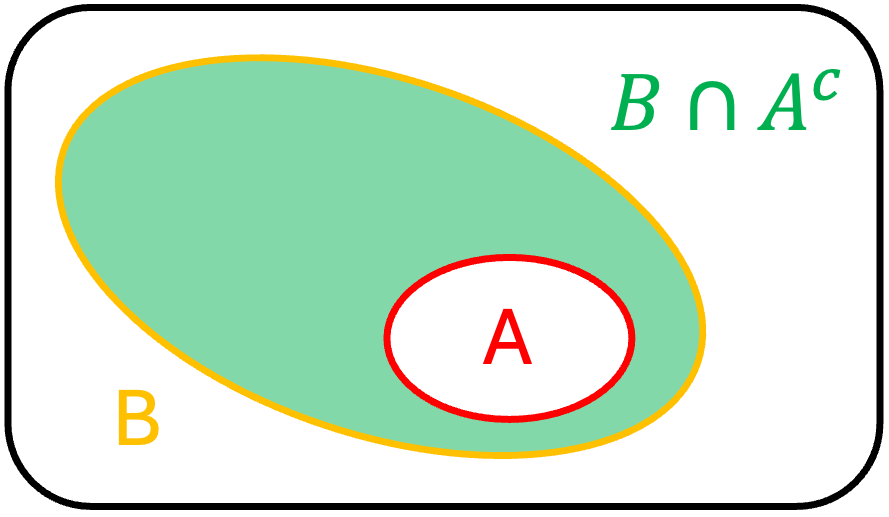
\includegraphics[width=0.2\textwidth]{Media/Dim_1.7.png}
        \end{center}
        $\overset{\text{P.1}}{\Rightarrow}\;\;\; \mu(B) = \mu(A \cup (B \cap A^c)) = \mu(A) + \mu(B \cap A^c)) \geq \mu(A)$ \\
        In quanto la misura è non negativa.
    \end{itemize}
    
    \end{dimostrazione}
\end{proposizione}

\vspace{\baselineskip}
\subsection{Alcune misure fondamentali}
\begin{itemize}[label=\(\bigstar\), align=left, labelsep=0.5em, labelwidth=!, leftmargin=0pt]
\item Una misura fondamentale nella Teoria della misura è la \textbf{Massa di Dirac} in un punto $\alpha_0$.\\
Preso  $\alpha_0 \in E$, si ha che $\forall A \subseteq E$:
\[ \mu(A) = 
\begin{cases} 
    1, & \text{se } \alpha_0 \in A \\ 
    0, & \text{se } \alpha_0 \notin A
\end{cases}
\]
Questa risulta essere una misura finita.\\
Se infatti prendo $E = \mathbb{R};\alpha_0 = 0;A = [-3, 5)\quad \Rightarrow \quad \mu(A) = 1$\\
Se prendessi invece $B = [-3, -1)\quad \Rightarrow \quad \mu(B) = 0$.\\
Notiamo inoltre che se scrivessi $\mathbb{R}$ come fatto nell'esempio della misura di Lebesgue, non avrei insiemi disgiunti, e di conseguenza non potrei dire che $\mathbb{R}$ ha misura infinita.
\item Consideriamo adesso un'altra misura: la \textbf{Misura Puramente Atomica}. Preso $E$ numerabile, ovvero: $E = \set{\alpha_n : n\geq 0}$, associo a $(\alpha_n)_n$ un'altra successione $(p_n)_{n\geq 0}$ tale che $p_n\geq0$. Siccome $E$ è misurabile avremo che \[A = \bigcup_{k:\alpha_k\in A}\{\alpha_k\}\]
Posso quindi definire la misura:
\[\mu(A) = \sum_{k:\alpha_k\in A} p_k\]
È come se si vedono gli elementi della successione che sono in $A$, e ne sommo i relativi pesi $p_k$; essendo quest'ultimi non negativi la serie non dipenderà dall'ordine, quindi avremo o convergenza o divergenza.
\newpage
\begin{esempio}
    Caso finito.\\
    \[E  = \{1, ..., 6\} \xrightarrow{Associo} \left(\frac{1}{6}, \frac{1}{6}, \frac{1}{6}, \frac{1}{6}, \frac{1}{6}, \frac{1}{6}\right)
    \]
    \[\{\alpha_1, ..., \alpha_6\} \xrightarrow{Associo} (p_1, ..., p_6)\]
    Sia $A\subseteq E: A = \{2, 4, 6\}$\\
    \[\Rightarrow \mu(A) = \sum_{k:\alpha_k\in A} p_k = p_2 + p_3 + p_6 = \frac{1}{6} + \frac{1}{6} + \frac{1}{6} = \frac{1}{2} \]
    Questo caso risulta parecchio semplificato perché l'insieme è finito.
\end{esempio}

\begin{esempio}
    Caso Numerabile.\\
    \[E = \mathbb{N}^* = \mathbb{N} \setminus\{0\} = \{\alpha_n : n\geq 1\} = \{n : n\geq 1\} \xrightarrow{Associo} p_n = n \quad \forall n\geq1\]
    Sia $A\subseteq E$, tale che $A = \{n_k:k\geq1\}$, ovvero che sia una sotto-successione. La misura in questione risulta essere quindi:
    \[\mu(A) = \sum_{k=1}^\infty p_k = \sum_{k=1}^\infty \frac{1}{n_k}\]
    La quale diverge se la si calcola in $E$, rendendo la misura \textit{non} finita:
    \[\mu(E) = \sum_{n=1}^\infty p_n = \sum_{n=1}^\infty \frac{1}{n} = +\infty\]
    Tuttavia si può partizionare l'insieme $E$, andando ad identificare gli insiemi $E_k = \{k\}$, avendo così che $\mu(E_k) = 1/k < +\infty\quad \forall k \geq 1$.\\
    Se inoltre ci si accorge che \[\bigcup_{k\geq1} E_k = \bigcup \{k\} = \mathbb{N}^* = E\]
    allora si può concludere che $\mu$ sia una misura $\sigma$-finita.\\
    \\
    Questo esempio dimostra un fatto fondamentale: se ho una successione numerabile, posso sempre invadere l'insieme nella modalità appena eseguita, verificando sempre che $\mu$ sia una misura $\sigma$-finita.
\end{esempio}

Si noti che preso $E = \{\alpha_n:n\geq1\}$, ovvero un insieme numerabile, e $(p_n)_{n\geq1}:\quad p_n\geq0\quad \forall A\in\mathcal{P}(E)$, allora si avrà sempre che
\[\mu(A) = \sum_{k:\alpha_k\in A} p_k\]
e di conseguenza, si avrà che: \(\mu(E) = \sum_{n} p_n\) dimostrando che
\(\mu \text{ è finita} \iff \sum_{n} p_n < +\infty\).\\
\\
Si noti inoltre che possiamo scrivere la misura come:
\[\mu(A) = \sum_{k:\alpha_k\in A} p_k = \sum_{n=1}^\infty p_n \cdot \delta_{\alpha_n}(A)\]
ossia che possiamo vederla come una \textit{combinazione lineare} di masse di Dirac.

\item La \textbf{Misura di Lebesgue} è già stata introdotta, tuttavia questa può essere estesa anche a casi non monodimensionali. Si ha infatti che:
\begin{enumerate}
    \item Su $\mathbb{R}:\qquad \;\,m_1([a, b)) = b-a$ \hfill \textit{(Lunghezza)}
    \item Su $\mathbb{R}^2:\qquad m_2(B(0, r)) = \pi r^2$ \hfill \textit{(Area)}
    \item Su $\mathbb{R}^3:\qquad m_2(B(0, r)) = \frac{4}{3}\pi r^3$ \hfill \textit{(Volume)}
\end{enumerate}
Anticipiamo che $m$ non può essere definita su tutti i sottoinsiemi di $\mathbb{R}$ perché sono "troppi"; non potremo quindi usare come $\sigma$-algebra $\mathcal{P}(\mathbb{R})$. Più avanti approfondiremo la questione, andando ad individuare una $\sigma$-algebra che sia adatta ai nostri scopi.
\end{itemize}
